%part 3

	\chapter{Регулирование критической энергии методом резонансной вариации дисперсионной функции}\label{ch:resonant}

\par Эта глава посвящена общим подходам при проектировании резонансной структуры с варьируемой критической энергией. Также рассматривается адаптации структуры коллайдера NICA с поднятой критической энергией выше конечной энергии эксперимента для возможности осуществления столкновения легких поляризованных пучков протонов и дейтронов на SPD детекторе.

\par	Альтернативным способом, который применяется для того чтобы избегать потери стабильности, является создание или модификация структуры с заведомо большим значением критической энергии. Такая структура носит название 'резонансной' \cite{senichev:resonant}, \cite{senichev:construction}, впервые была предложена при проектировании каонной фабрики \cite{kaon_tr} и других установках мирового уровня Neutrino Factory в CERN \cite{neutrino_tr} и было реализовано в J-PARC для главного кольца \cite{JHP_tr}, \cite{J-PARK_tr}. Принципиальным отличием от регулярной структуры является обеспечение резонансного условия для количества суперпериодов и частоты бетатронных колебаний в горизонтальной плоскости. Однако, это справедливо только для не полностью регулярных структур, а содержащих регулярную модуляцию градиента квадруполей или кривизны орбиты. В таком случае, происходит изменение оптических функций ускорителя и варьирование критической энергии выше энергии эксперимента, в том числе до комплексных значений, полностью убирая зависимость установки от дополнительных процедур преодоления. Такой подход позволяет получить нулевую дисперсию на прямых участках в силу подавления дисперсии на поворотных арках, путём выбора целого числа бетатронных колебаний и создания ахромата первого порядка. Кроме того, в подобной структуре может быть легко реализован и ахромат второго порядка расстановкой секступолей через один суперпериод. Подобный подход способствует достижению достаточного значения динамической апертуры.

\begin{comment}
В эксперименте по столкновению тяжелых ионов золота c максимальной энергией $E_{exp}=4.5$ ГэВ/нуклон критическая энергия магнитооптической структуры коллайдера составляет $E_{tr}^{Au-Au}=5.7$\ ГэВ ($\gamma_{tr}^{Au-Au}=7.1$). Такое значение критической энергии было достигнуто выбором частоты бетатронных колебаний в горизонтальной плоскости $\nu_x\approx\gamma_{tr}^{Au}>\gamma_{max}^{Au}\approx7.1$, которая  при условии регулярности структуры арок, состоящих из одинаковых ячеек ФОДО, должна быть больше максимального значения фактора Лоренца во всем интервале энергий.
\end{comment}

\par Как было показано в Главе \ref{ch:dual}, структура коллайдера NICA проектировалась как дуальная для работы в двух модах: для экспериментов с тяжелыми ионами $^{\mathbf{79}}{\mathbf{Au}}_{\mathbf{197}}$ и для экспериментов с поляризованными протонами и дейтронами $\mathbf{p, d}$. В этом случае проблем с прохождением критической энергии не возникает, что было изначально учтено при проектировании. Однако, спроектированная и построенная регулярная структура, выбранная для тяжелоионной программы имеет фиксированное значение критической энергии и является характеристикой конкретной установки, то есть не отличается для разного сорта частиц. Характер поведения тяжелых ионов и легких частиц, существенно отличается с точки зрения внутрипучкового рассеяния. Для протонного пучка с интенсивностью $1\times10^{12}$ время внутрипучкового нагрева возрастает примерно в 10 раз по сравнению с пучками ионов золота с интенсивностью $2.2\times10^{9}$. Поэтому критическая энергия может подниматься за счет вариации дисперсии без опасения влияния внутрипучкового рассеяния. За счет резонансной модуляции дисперсионной функции коэффициент диффузии для внутрипучкового рассеяния возрастает в 2-3 раза, что не критично как при охлаждении протонов во время накопления, так и при их группировке на энергии эксперимента.

\par Как было показано в Главе \ref{ch:transition}, при прохождении через критическую энергию $\gamma_{\text{tr}}$ развивается продольная неустойчивость для интенсивных сгустков. Пороговый ток ее развития $I_{\text{th}}\sim\eta$ пропорционален коэффициенту расширения орбиты, который стремится к нулю в первом приближении при $\gamma=\gamma_{\text{tr}}=7.1$. Темп ускорения протонов при прохождении через критическую энергию при использовании индукционного ускорения в станции ВЧ1 составляет $\dv{\gamma}{t}=0.2~\text{c}^{-1}$. Этот темп слишком мал, чтобы полностью избежать развития неустойчивости при приближении релятивистского фактора к $\gamma_{\text{tr}}$. Чтобы исключить при ускорении протонов прохождение через критическую энергию, для протонной моды должна быть реализована новая оптическая структура колец вместо оптической структуры тяжелоионной моды. В этой оптической структуре критическая энергия должна быть выше максимальной энергии протонов при работе коллайдера на эксперимент.

\par Максимальная магнитная жесткость поворотных магнитов постоянна $R_{\text{arc}}\cdot B_{\text{bend}}=\frac{A\cdot m c\gamma\beta}{eZ}\approx45~\text{Тл/м}$. В силу того, что отношения массы к заряду $\left(A/Z\right)_{\text{p}}=1/1=1$, для ионов золота $\left(A/Z\right)_{\text{Au}}=197/79=2.2$. Тем самым, определяется максимально возможная энергия для протонов $E_{\text{max}}^{\text{p}}~=~12.4$~ГэВ ($\gamma_{\text{p}}=14.3$), следовательно критическая энергия должна быть не менее ($\gamma_{\text{tr}}~=~15-16$), что заведомо выше критической энергии для ионной регулярной структуры $E_{\text{tr}}^{\text{Au}}=5.7$\ ГэВ ($\gamma_{\text{tr}}^{\text{Au}}=7,1$).

\par В данной главе будут приведен краткое теоретической обоснование применения метода резонансной структуры. Теоретический метод был развит в работе \cite{senichev:resonant}, а его применение для современных ускорительных установок рассмотрено в работе \cite{senichev:construction}. Изучена возможность адаптации регулярной магнитооптической структуры главного кольца NICA к резонансной. А также анализ полученной структуры с точки зрения компенсации нелинейных эффектов, компенсации хроматичности и  динамической апертуре.
  
\section{Введение суперпериодической модуляции}\label{sec:transition_variation/methods/resonant}

\par Здесь будет приведено кратное теоретическое обоснование метода резонансных структур, применяемых для обеспечения вариации критической энергии. Исходя из уравнения \ref{eq:alpha} коэффициент расширения орбиты $\alpha$ зависит как от дисперсионной функции $D(s)$, так и радиуса кривизны орбиты $\rho(s)$, таким образом вариация критической энергии может быть достигнута путем введения независимой модуляции обеих функций.

\par Уравнение для дисперсионной функции с бипериодической переменной фокусировкой описывает поведение с учётом влияния градиентов в квадрупольных линзах, а также радиуса кривизны орбиты \cite{senichev:resonant}

\begin{equation}
\dv[2]{D}{s}+\left[K(s)+\varepsilon k(s)\right]D=\frac{1}{\rho(s)} ,
\label{eq:disp_eq}
\end{equation}

\noindent где $K\left(s\right)=\frac{e}{p}G\left(s\right), \varepsilon k\left(s\right)=\frac{e}{p}\Delta G\left(s\right), G\left(s\right)$ – градиент магнитооптических линз, $\Delta G\left(s\right)$ – суперпериодическая модуляция градиента, $p=\beta\gamma m_0 c$ – импульс частицы. Суперпериод определяется как совокупность нескольких периодов. Функция $K\left(s\right)$ имеет периодичность одного периода фокусирующей ячейки $L_{c}$, $k(s)$ и $\rho(s)$ имеет периодичность суперпериода $L_{\text{s}} = n \cdot L_{\text{c}}$.

Разложение в ряд  Фурье для зеркального суперпериода может быть осуществлено только по косинусам

\begin{equation}
\varepsilon k\left(\phi\right)=\sum_{k=0}^{\infty}g_{k}\cos(k\phi),
\label{eq:superperiodicity_fourier}
\end{equation}

\noindent где $\phi=\frac{2\pi}{L_s}s$ -- угловая продольная координата, $k$-ая гармоника:
\begin{equation}
g_k=\frac{1}{B\bar{R}} \frac{1}{\pi} \int_{-\pi}^\pi \Delta G \cos k \phi d \phi,
\end{equation}
\noindent где $B\bar{R}$ -- магнитная жесткость.

\noindent Радиус кривизны орбиты также может быть разложен в ряд Фурье по косинусам

\begin{equation}
\frac{1}{\rho(\phi)}=\frac{1}{\bar{R}}\left(1+\sum_{n=1}^{\infty} r_n \cos n \phi\right),
\end{equation}

\noindent где $n$-ая гармоника

\begin{equation}
r_n=\frac{\bar{R}}{\pi} \int_\pi^{-\pi} \frac{\cos n \phi}{\rho(\phi)} d \phi.
\end{equation}

\noindent Полученные разложения могут быть подставлены в уравнение \ref{eq:disp_eq}, из которого получено необходимое точное решение для дисперсионной функции $D(s)$. Таким образом, окончательно для коэффициента уплотнения орбиты одного суперпериода получено выражение в общем виде, разложенное до второго порядка

\begin{equation}
\begin{gathered}
\alpha_{\text{s}}=\frac{1}{\nu^2}\left\{1+\frac{1}{4}\left(\frac{\bar{R}}{\nu}\right)^4 \sum_{k=-\infty}^{\infty}\right.
\frac{g_k^2}{(1-k S / \nu)\left[1-(1-k S / \nu)^2\right]^2}+ \\
+\frac{1}{4} \sum_{k=-\infty}^{\infty} \frac{r_k^2}{1-k S / \nu} -\frac{1}{2}\left(\frac{\bar{R}}{\nu}\right)^2 \sum_{k=-\infty}^{\infty} \frac{r_k g_k}{(1-k S / \nu)\left[1-(1-k S / \nu)^2\right]} - \\
-\frac{1}{2}\left(\frac{\bar{R}}{\nu}\right)^2 \sum_{k=-\infty}^{\infty} \frac{r_k g_k}{1-(1-k S / \nu)^2}
\left.+O\left(g_k^i, r_k^j, i+j \geq 3\right)\right\},
\end{gathered}
\label{eq:alpha_general}
\end{equation}

\noindent где ${\overline{R}}_{\text{arc}}$ -- усредненное значение кривизны, $\nu=\nu_{x}$ -- количество горизонтальных бетатронных колебаний на длине арке, $S$ -- количество суперпериодов на длине арки. В случае отсутствия суперпериодической модуляции и модуляции кривизны орбиты $g_k=0, r_n=0 \  \forall k,n$, формула \ref{eq:alpha_general} принимает вид $\alpha_{\text{s}}=\frac{1}{{\gamma_{\text{tr}}}^2}=\frac{1}{{\nu_x}^2}$, что соответствует случаю регулярной структуры и наглядно видно, что  $\gamma_{\text{tr}}\sim\nu_x$. Для поднятия критической энергии необходимо уменьшить коэффициент $\alpha_{\text{s}}=\frac{1}{{\gamma_{\text{tr}}}^2}$, а значит выражение под знаком суммы в ур.\ref{eq:alpha_general} должно быть отрицательным. Это реализуемо при условии $kS/\nu_{x}>1$, когда осуществлена либо модуляция градиентов квадруполей $g_k\not=0$, либо радиуса $r_n\not=0$.

\par Ранее все формулы были приведены для суперпериода, а не для всего кольца коллайдера. Введение прямых участков уменьшает степень модуляции дисперсионной функции. Усреднение дисперсии по более длинной орбите автоматически уменьшает ее значение, а значит уменьшает коэффициент уплотнения орбиты для всего ускорителя, результирующее значение критической энергии $\gamma_{\text{tr}}^{\text{total}}$ увеличивается и определяется выражением:

\begin{equation}
\gamma_{\text{tr}}^{\text{total}}=\gamma_{\text{tr}}^{\text{arc}}\sqrt{\frac{S\cdot L_{\text{s}}+L_{\text{str}}}{S\cdot L_s}},
\label {eq:gamma_tr_modulated}
\end{equation}

\noindent где $L_{\text{s}}$ -- длина суперпериода, $L_{\text{str}}$ -- длина бесдисперсионных прямых секций.

	\section{Построение резонансной структуры на основе ячеек ФОДО, ФДО, ОДФДО}\label{sec:transition_variation/methods/FODO_FDO}

Исходя из уравнения \ref{eq:alpha_general}, в случае отсутствия модуляции кривизны орбиты $r_n=0, \ \forall n$ для одного суперпериода в первом приближении (при $k=1$) коэффициент расширения орбиты приобретает вид
	
\begin{equation}
\begin{aligned}
\alpha_s= & \frac{1}{\nu^2}\left\{1+\frac{1}{4(1-k S / \nu)}\left(\frac{\bar{R}}{\nu}\right)^4 \frac{g_k^2}{\left[1-(1-k S / \nu)^2\right]^2}\right\}.
\end{aligned}
\label{eq:alpha_gradient}
\end{equation}

\noindent Таким образом, доступным средством вариации критической энергии, является только модуляция градиента квадрупольных линз по длине суперпериода. Одинаковые элементы, расположенные в различных местах арки объединяют в одно семейство. На рис. \ref{fig:superperiod_3FODO} изображен один суперпериод, который состоит из 3-х ФОДО ячеек, c двумя семействами фокусирующих квадруполей (QF1 и QF2) и одним семейством дефокусирующих (QD).

\begin{figure} [h!]
   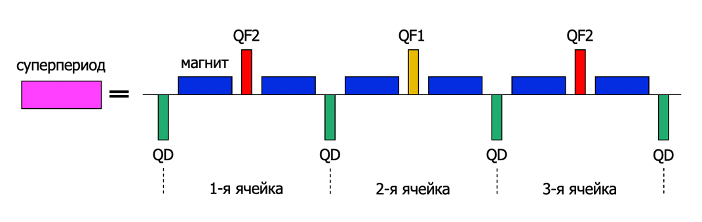
\includegraphics[width=1\columnwidth]{2_superperiod.png}
   \caption{Суперпериод, состоящий из 3-х ФОДО ячеек. QF1, QF2 -- фокусирующие квадруполи, QD -- дефокусирующие квадруполи, B -- поворотный магнит.}
   \label{fig:superperiod_3FODO}
\end{figure}
	
\par Суперпериод может быть образован на основе синглетных ФОДО ячейках, дублетных ФДО ячейках, а также триплетных ОДФДО (рис.\ref{fig:fodo_fdo_odfdo} a,б,в). Рассмотрим структуры поворотных арок на 180 градусов без модуляции кривизны (рис.\ref{fig:fodo_fdo_odfdo} г, д, е), образованных из соответствующих ячеек. Из полученных суперпериодов также образуется резонансная магнитооптическая структура путем только модуляции градиента (рис.\ref{fig:fodo_fdo_odfdo} ж, з, и). Резонансная структура образуется путем вариации параметров регулярной структуры.

\begin{figure} [h!]

   \includegraphics*[width=.32\columnwidth]{2_twiss_fodo_cell.pdf}
   \includegraphics*[width=.32\columnwidth]{2_twiss_fdo_cell.pdf}
   \includegraphics*[width=.32\columnwidth]{2_twiss_odfdo_cell.pdf}

   \includegraphics*[width=.32\columnwidth]{2_twiss_fodo_resonant.pdf}
   \includegraphics*[width=.32\columnwidth]{2_twiss_fdo_resonant.pdf}
   \includegraphics*[width=.32\columnwidth]{2_twiss_odfdo_resonant.pdf}

   \caption{Твисс-параметры $\beta_{x,y}$, $D_{x}$. Сверху -- для ячеек для сигнлетной ФОДО, дублетной ФДО, триплетной ОДФДО ячеек; посредине -- регулярная структура; снизу -- резонансная.}
   \label{fig:fodo_fdo_odfdo}
\end{figure}

\par Качественное отличие в пространственном распределении Твисс-параметров $\beta_{x}$, $\beta_{y}, D_{x}$ является ключевым для соответствующей оптимизации структуры.
Как видно из приведенных структур, суперпериод, основанный на синглетных ФОДО ячейках может иметь ряд преимуществ.

\noindent Хроматичность зависит от величины градиентов в квадруполях, секступолях, а также местах их расположения \cite{lee}

\begin{equation}
\begin{aligned}
& C_x=-\frac{1}{4 \pi} \oint \beta_x\left[K_x(s)-S(s) D(s)\right] \textrm{d} s, \\
& C_y=-\frac{1}{4 \pi} \oint \beta_z\left[K_y(s)+S(s) D(s)\right] \textrm{d} s.
\end{aligned}
\end{equation}

\noindent Отсюда видно, что, во-первых, для подавления хроматических эффектов в ФОДО-ячейке, требуются меньшие градиенты в секступольных линзах. Во-вторых, более простой способ коррекции и тонкой настройки набега бетатронных частот в обеих плоскостях, а также коэффициента расширения орбиты. Таким образом, является более предпочтительной по сравнению с аналогичными.

	\section{Регулярная ФОДО структура с суперпериодической модуляцией градиентов линз}\label{sec:transition_variation/methods/FODO}

\begin{figure}
   \includegraphics*[width=.49\columnwidth]{2_twiss_3FODO_regular}
   \includegraphics*[width=.49\columnwidth]{2_twiss_3FODO_modulated}
   \caption{Твисс-параметры 3-х ячеек. Слева – регулярная структура без модуляции, справа – модулированная c введением суперпериодичности, глубина модуляции 24\%.}
   \label{fig:twiss_3FODO}
\end{figure}

\par Поскольку квадрупольная фокусирующая структура поворотных арок коллайдера NICA состоит из ФОДО ячеек, рассмотрим возможность адаптации регулярной структуры к резонансной. На рис. \ref{fig:twiss_3FODO} приведены 3 ФОДО ячейки, первая – используется в регулярной тяжелоионной структуре, в этом случае модуляция отсутствует, вторая – модулированная структура,  которая и образует один суперпериод. В обоих случаях частота бетатронных колебаний для одного суперпериода $\nu_{x,y}=0.75$, таким образом для 4-х суперпериодов частота $\nu_{x,y\ \text{arc}}=3$, что удовлетворяет ранее рассмотренному условию $S=4, \nu_x=3$.

Глубина модуляции определяется соотношением градиентов двух различных фокусирующих семейств. Для приведенного на правом рисунке рис. \ref{fig:twiss_3FODO} $G_{\textrm{QF1}}=27.7$ Тл/м, $G_{\textrm{QF2}}=21.0$ Тл/м. Таким образом глубина модуляции:

\begin{equation}
H=\frac{G_{\textrm{QF1}}-G_{\textrm{QF2}}}{G_{\textrm{QF1}}}=24\%
\label {eq:modulated_coeff}
\end{equation}

\par Первая гармоника является определяющей и для 12 ФОДО ячеек реализуемо условие $S=4, \nu_x=3$, где 3 ФОДО ячейки объединены в один суперпериод. Таким образом, благодаря набегу бетатронных колебаний кратному $2\pi$, в нашем случае $6\pi$, арка имеет свойства ахромата первого порядка. Благодаря этому свойству может быть подавлена дисперсия без дополнительных усилий.

\par Для арки, составленной из 4-х одинаковых суперпериодов с критической энергией  на арке $\gamma_{\text{tr}}^{\text{arc}}=\ 10$, по формуле \ref{eq:gamma_tr_modulated} для всего кольца получаем $\gamma_{\text{tot}}^{\text{arc}}\ \approx\ 15.9$. Однако, конечная арка будет нерегулярной в силу необходимости подавления дисперсии на краях арки, а значит в конкретном реальном случае значение критической энергии будет несколько отличаться.

\section{Подавление дисперсии на краях поворотных арок}\label{sec:transition_variation/disp_supperssion}

\par Важным требованием при проектировании магнитооптической структуры является обеспечение нулевого значения дисперсии на прямых участках для обеспечения движения частиц вдоль равновесной орбиты на этих участках. Это условие легко реализуется при подавлении дисперсии и её производной на концах поворотной арки. Рассматривается 4 варианта подавления дисперсии:

\begin{enumerate} 
\item	Полносью регулярная арка. \ Регулярная арка состоящая из 4-х одинаковых суперпериодов. При набеге фазы на арке кратному $2\pi$ подавление дисперсии происходит в силу регулярности;
\item Регулярная арка с применением методики отсутствующих магнитов на двух крайних ячейках арки, что показано на рис. \ref{fig:2_disp_supp}.
\item В структуре с отсутствующими магнитами при переходе к резонансной оптике, подавление дисперсии возможно при помощи крайних суперпериодов. В этому случае при набеге фазы на арке не кратному $2\pi$ необходимо дополнительно добавить подавители дисперсии на краях арки, а именно двух крайних ФОДО ячеек. Две крайние ФОДО ячейки отличаются наличием и в этих ячейках квадруполи QFE1 и QFE2 также имеют отличные градиенты от основных квадруполей арки и подбираются таким образом, чтобы подавить дисперсию.
\item В структуре с отсутствующими магнитами при переходе к резонансной оптике, также возможно подавление дисперсии всей аркой, при помощи выбора градиентов квадруполей двух семейств. Этот случай отличается тем, что все квадруполи арки принадлежат первому, либо второму семейству и подавление дисперсии также обеспечивается только 2-мя семействами.
\end{enumerate} 

\noindent Дефокусирующие же квадруполи во всех случаях принадлежат только одному семейству QD. Рассмотрим представленные случаи  более подробно.

\begin{figure} [h!]
	\center
	\includegraphics*[width=.6\columnwidth]{2_disp_supp}
	\caption{Подавление дисперсии в тяжелоионной структуре.}
	\label{fig:2_disp_supp}
\end{figure}

\subsection{Полностью регулярная магнитооптическая структура}\label{subsec:transition_variation/disp_supperssion/regular}

\par Требование подавления дисперсии легко реализуемо в случае создания регулярных поворотных арок, составленных из одинаковых суперпериодов. В этом случае, обеспечив нулевое значение дисперсии $D=0$ (а также производной дисперсии $D{\prime}=0$) на входе в арку, в силу регулярности на выходе из арке также будут нулевые значения дисперсии и её производной, а следовательно и на всем прямом участке. Однако, учитывая особенность структуры коллайдера NICA, наличие отсутствующих магнитов на двух крайних ячейках не дает возможность создать полностью регулярную арку из 4-х одинаковых суперпериодов.

\begin{figure} [h!]
   \center
   \includegraphics*[width=1.\columnwidth]{2_supp_scheme_regular.png}
   \includegraphics*[width=1.\columnwidth]{2_supp_Twiss_regular.png}
   \includegraphics*[width=1.\columnwidth]{2_supp_elem_regular.png}
   \caption{Подавление дисперсии в регулярной структуре.}
   \label{fig:2_disp_supp_full_regular}
\end{figure}
	
\subsection{Подавление дисперсии при помощи крайних суперпериодов}\label{subsec:transition_variation/disp_supperssion/ES}

\par	
\begin{figure} [h!]
   \center
   \includegraphics*[width=1.\columnwidth]{2_supp_scheme_ES.png}
   \includegraphics*[width=1.\columnwidth]{2_supp_Twiss_ES.png}
   \includegraphics*[width=1.\columnwidth]{2_supp_elem_ES.png}
   \caption{Подавление дисперсии в тяжелоионной структуре.}
   \label{fig:2_disp_supp_ES}
\end{figure}		

\par В этому случае выбор значения градиентов квадруполей арки определяется двумя факторами:
	а) получение необходимого значения критической энергии на всем кольце коллайдера, что соответствует $\gamma_{\text{tr}}\sim15-16$;
	б) обеспечение количество бетатронных колебаний на арке $\nu_{\text{arc}}=3$ в обоих плоскостях, тем самым удовлетворив резонансному условию при количестве суперпериодов $S=4$. Исходя из этих условий модулируем суперпериод с набегом фазы на суперпериоде $\nu_{\text{s}}=0.75$ в обоих плоскостях.

\par Коллайдер также состоит из 2-х арок и 2-х прямых участках, соединяющих арки. В центре прямых участков имеются точки столкновения, где нужно обеспечить малое значение бета-функции для достижения требуемой светимости. В крайнем суперпериоде применяется метод отсутствующих магнитов в 2-х ячейках, тем самым делая арки коллайдера не регулярными и возникает необходимость подавления дисперсии на прямых участках при помощи введения 2-х дополнительных семейств квадруполей QFE1 и QFE2 на краю арки, параметры Твисса изображены на рис. \ref{fig:2_disp_supp_ES}. В результате значение критической энергии подобрано таким образом, что $\gamma_{\text{tr}}=15.6$, а количество колебаний на арке: $\nu_{x,\ \text{arc}}=3.01,\ \nu_{y,\ \text{arc}}=3.01$.

\subsection{Подавление дисперсии всей аркой, при помощи выбора градиентов квадруполей двух семейств.}\label{subsec:transition_variation/methods/disp_supperssion_AS}	

Данный способ показывает возможность подавления дисперсии на прямых участках при помощи только двух семейств фокусирующих квадруполей. Тут важно учесть, как и в первом случае выполнить:
	а) получение необходимого значения критической энергии на всем кольце коллайдера, что соответствует $\gamma_{\text{tr}}\sim15-16$;
	б) только при помощи квадруполями двух семейств подавить дисперсию на прямых участках.

\begin{figure} [h!]
	\center
	\includegraphics*[width=1.\columnwidth]{2_supp_scheme_AS.png}
	\includegraphics*[width=1.\columnwidth]{2_supp_Twiss_AS.png}
	\includegraphics*[width=1.\columnwidth]{2_supp_elem_AS.png}
	\caption{Подавление дисперсии в тяжелоионной структуре.}
	\label{fig:2_disp_supp_AS}
\end{figure}
	
\par Изначально выбирается суперпериод, как и в первом случае с набегом на суперпериоде $\nu_s=0.75$. Тем самым получаем значения квадруполей QF1 и QF2 для всей арки, в том числе и на краях. Однако, получается, что дисперсия на прямых участках оказывается не подавленной. Для подавления значения градиентов квадруполей изменяется, но в таком случае набег фазы на арке становится равен $\nu_{x,\ \text{arc}}=2.72178$,\ $\nu_{y,\ \text{arc}}=2.99884$, то есть в x–плоскости не кратен $2\pi$. В этом случае для достижения требуемого значения критической энергии необходимо обеспечить большую модуляцию градиентов квадруполей, чем в случае подавления дисперсии крайними суперпериодами. Принципиальная схема показана на рис. \ref{fig:DA_AS_dpp}. Для полученной нерегулярной арки значение критической энергии $\gamma_{\text{tr}}^{\text{arc}}=\ 10$.

\section{Исследование динамической апертуры в синхротроне с учетом требуемой модуляции дисперсионной функции для повышения критической энергии}

\begin{figure} [h!]
	\center
	\includegraphics*[width=0.49\columnwidth]{2_ES_x_dpp0.png}
	\includegraphics*[width=0.49\columnwidth]{2_ES_y_dpp0.png}
	\includegraphics*[width=0.49\columnwidth]{2_ES_x_dpp0,3.png}
	\includegraphics*[width=0.49\columnwidth]{2_ES_y_dpp0,3.png}
	\includegraphics*[width=0.49\columnwidth]{2_ES_x_dpp0,5.png}
	\includegraphics*[width=0.49\columnwidth]{2_ES_y_dpp0,5.png}
	\caption{Динамическая аппретура для случая плавления дисперсии крайними квадруполями. 
		Слева – $x$-плоскость; справа – $y$-плоскость.}
	\label{fig:DA_ES_dpp}
\end{figure}	

\begin{figure} [h!]
   \center
   \includegraphics*[width=0.49\columnwidth]{2_AS_x_dpp0.png}
   \includegraphics*[width=0.49\columnwidth]{2_AS_y_dpp0.png}
   \includegraphics*[width=0.49\columnwidth]{2_AS_x_dpp0,3.png}
   \includegraphics*[width=0.49\columnwidth]{2_AS_y_dpp0,3.png}
   \includegraphics*[width=0.49\columnwidth]{2_AS_x_dpp0,5.png}
   \includegraphics*[width=0.49\columnwidth]{2_AS_y_dpp0,5.png}
   \caption{Динамическая апертура в случае подавление дисперсии двумя семействами квадруполей.
Слева – $x$-плоскость; справа – $y$-плоскость.}
   \label{fig:DA_AS_dpp}
\end{figure}

\par Выбор нечетного значения частоты на арке $\nu_{x,\ \text{arc}}=3$ и четного значения суперпериодичности арки $S=4$ замечателен еще и тем, что позволяет компенсировать нелинейный вклад секступолей внутри арки. Добавление секступолей, подавляющих хроматичность внутри арки делает арку ахроматом второго порядка, что убирает зависимость бетатронных колебаний от импульса и способствует сохранению динамической апертуры в большом диапазоне энергий. В этом случае набег фазы радиальных колебаний между ячейками, расположенными в разных половинках арки и разделенных $S/2$ числом суперпериодов равен:

\begin{equation}
2\pi\cdot\frac{\nu_{\text{arc}}}{S_{\text{arc}}}\cdot\frac{S_{\text{arc}}}{2}=2\pi\cdot\frac{\nu_{\text{arc}}}{2}=\pi+2\pi n,\
\label{eq:chrom_period}
\end{equation}

\noindent что соответствует условию компенсации нелинейного влияния секступолей в первом приближении во всей арке. Это замечательное свойство также относится к высшим мультиполям в квадруполях и отклоняющих магнитах. Эта связь через число суперпериодов $S_{\text{arc}}/2$ называется длинной связью.

\section*{Выводы}
\par Рассмотрена методика вариации критической энергии методом модуляции градиента квадрупольных линз на арках. Такой случай предполагает раздельное питание квадруполей. Также учтена необходимость подавления дисперсии на краях арки в имеющейся структуре и подавление хроматичности на всем кольце коллайдера. Исследования выполнены в применении к ускорительному комплексу NICA, однако без потери общности, может применяться на различных установках.

\begin{enumerate}

\item Введение модуляции дисперсионной функции или радиуса кривизны орбиты приводит к вариации коэффициента уплотнения орбиты и как следствие критической энергии установки. Таким образом можно добиться повышенной критической энергии, выше энергии эксперимента, и также достижения комплексного значения;

\item Рассмотрены схемы подавления дисперсионной функции в резонансной структуре на краях поворотных арок. В случае полностью регулярной структуре это достигается путем выбора кратного набега фазы. При использовании метода отсутствующих магнитов ('missing magnet'), регулярность нарушается и возможно подавление как крайними ячейкам, так и только двумя семействами квадруполей;

\item Исследовано влияние нелинейных эффектов на динамическую апертуру в резонансной структуре. Для различных вариаций магнитооптики предложены оптимальные схемы расстановки секступолей.

\end{enumerate}

\FloatBarrier